\documentclass{beamer}

\usepackage{mpemath}
\usepackage{subcaption}
\usepackage[normalem]{ulem}
\usepackage{amsmath}
\usepackage{amssymb}
\usepackage{mathtools}
%\usepackage{pgf}
%\usepackage{pgfplots}
%\usepackage{tikz}
\usepackage{booktabs}
\usepackage{siunitx}
\usepackage{natbib}
\usepackage{tabularx}
\usepackage{multirow}
\usepackage{amsmath}
\usepackage{mathtools}
\usepackage{amssymb}
\usepackage{bbm}


%\usetikzlibrary{arrows,automata,backgrounds,positioning,decorations,intersections,matrix}

% *** Styles ***
\usetheme{Singapore}
\setbeamertemplate{navigation symbols}{}
% \usetheme[progressbar=frametitle]{metropolis}
% \usecolortheme{dolphin}
%\useinnertheme{circles}
%\usecolortheme{rose}
%\setbeamercovered{transparent}
\setbeamercovered{invisible}
\usefonttheme{professionalfonts}
%\usefonttheme[onlymath]{serif}
\setbeamertemplate{footline}[frame number]

\title{ROIL - Robust Offline Imitation Learning}
\author{\textbf{Gersi Doko$^1$}, Guang Yang$^2$, Daniel S. Brown$^2$, Marek Petrik$^1$}
\institute{Department of Computer Science \\ $1$ University of New Hampshire \\ $2$ University of Utah}
\date{}

\AtBeginSection[]{
	\begin{frame}
          \vfill
	\centering
	% \usebeamerfont{title}
        {\huge\bf \insertsectionhead}%
	\vfill
\end{frame}
}

\begin{document}

\frame{\titlepage}

\section*{Intro}

% - 8 minutes!!! Less than 8 slides aim for 2 slides intros, 3 slides idea, 2 slides results, 1-slide conclusion
% - The basic idea
% - Pictures!
% - One point to drive home all most all methods rely on a good u_e hat
%   - We propose a general technique to avoid estimating U_e hat
%   - don't even show the LP (if you do make sure you don't rely on it to make your point)
% - [ ] separate the images for the results into different slides too busy in one slide

\begin{frame}
\frametitle{Why Imitation Learning?}
	\begin{itemize}
		\item RL requires rewards 
		\vfill
		\item Rewards are hard to specify
		\vfill
		\item Often have access to expert demonstrations
		\vfill
		\item Imitation learning: Learn from demonstrations
	\end{itemize}
\end{frame}

\begin{frame}
  \frametitle{Inverse Reinforcement Learning}
  \begin{itemize}
    \item Leverage model dynamics to reduce sample complexity
    \vfill
    \item Aims to match experts occupancy frequency
    \vfill 
    \item Sensitive to state distribution
  \end{itemize}
\end{frame}

\begin{frame}
\frametitle{Off-Policy IRL}
\begin{figure}
  \begin{center}
  \begin{minipage}{0.45\linewidth}
    \centering
    \emph{On-Policy}\\
    \textbf{Expert's Occ Freq $u_e$}
    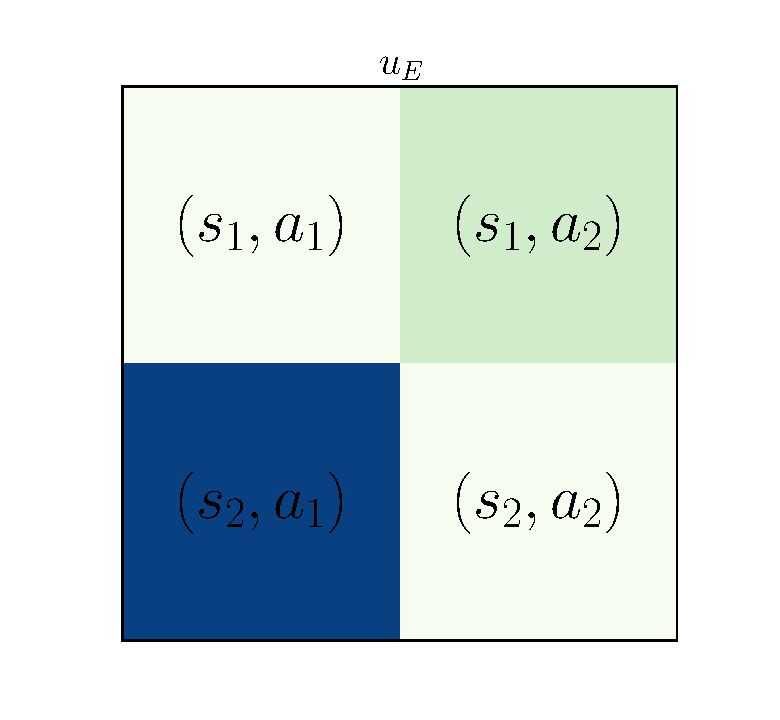
\includegraphics[width=\linewidth]{../../pres_roil/plots/all_state/ue.pdf}
    LPAL Return $= 86/87$
  \end{minipage}
  \begin{minipage}{0.45\linewidth}
    \centering
    \emph{Off-Policy}\\
    \textbf{Estimated Occ Freq $\hat{u}_e$}
    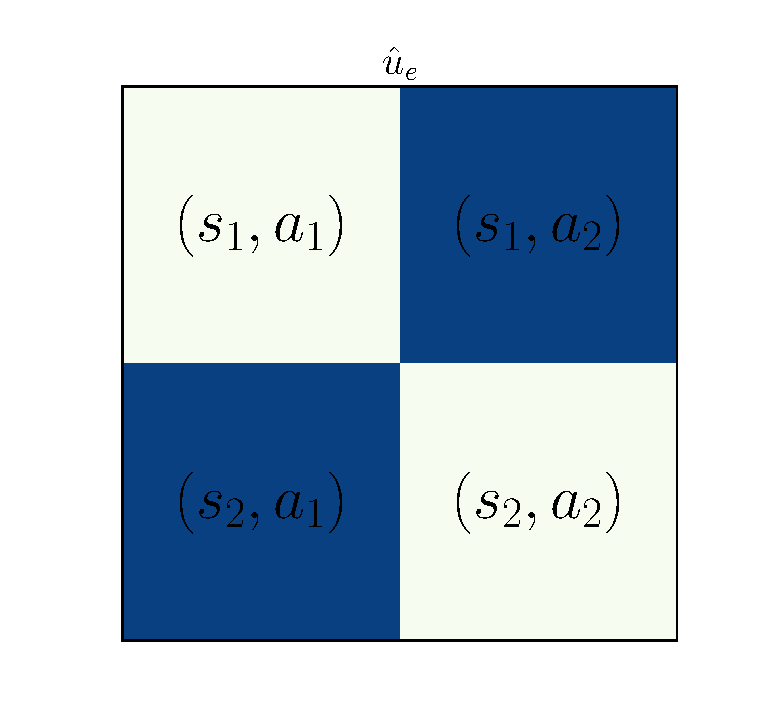
\includegraphics[width=\linewidth]{../../pres_roil/plots/all_state/uehat.pdf}
    LPAL Return $= 38/87$
  \end{minipage}
  \end{center}
\end{figure}
\end{frame}

\begin{frame}
\frametitle{Off-Policy IRL}
\begin{figure}
  \begin{center}
  \begin{minipage}{0.45\linewidth}
    \centering
    \emph{On-Policy}\\
    \textbf{Expert's Occ Freq $u_e$}
    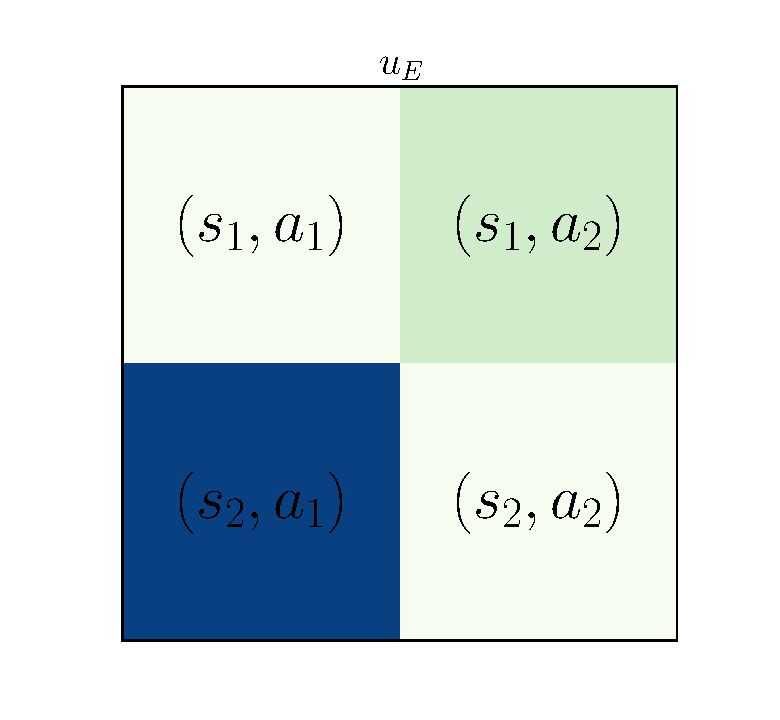
\includegraphics[width=\linewidth]{../../pres_roil/plots/all_state/ue.pdf}
    LPAL Return $= 86/87$ \\
    \textcolor{green}{\textbf{ROIL Return $= 79/87$}}
  \end{minipage}
  \begin{minipage}{0.45\linewidth}
    \centering
    \emph{Off-Policy}\\
    \textbf{Estimated Occ Freq $\hat{u}_e$}
    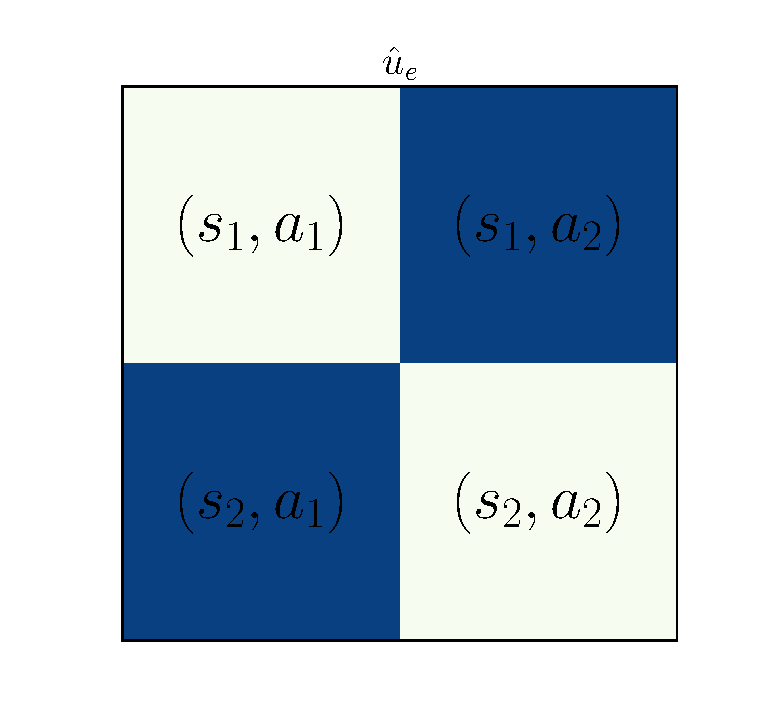
\includegraphics[width=\linewidth]{../../pres_roil/plots/all_state/uehat.pdf}
    LPAL Return $= 38/87$ \\
    \textcolor{green}{\textbf{ROIL Return $= 82/87$}}
  \end{minipage}
  \end{center}
\end{figure}
\end{frame}

\begin{frame}
	\frametitle{ROIL}
	\emph{Robust} method for \emph{off-policy} IRL

	\vfill
	\emph{Key Idea}
  \begin{itemize}
    \item Generate a convex set of consistent experts
    \item Formulate and minimize regret
  \end{itemize}
\end{frame}

\section*{ROIL}

\begin{frame}
	\frametitle{Our Approach}
	\textbf{Problem}: Find a policy $\pi$ that minimizes the regret with respect to the worst case expert consistent with the demonstrations $D_e$.
	\vfill
	\[ \textcolor{blue}{\min_{u^\pi \in \mathcal{U}}} \; \textcolor{red}{\max_{u_e \in \Upsilon}} \; \textcolor{purple}{\max_{r \in \mathcal{R}}} \;return(\textcolor{red}{u_e}, \textcolor{purple}{r}) - return(\textcolor{blue}{u^\pi}, \textcolor{purple}{r})\]
	\vfill
	\textbf{Solution}: Formulate as a linear program, we present ROIL and its many extensions
\end{frame}

\begin{frame}
  \vfill
  \begin{center}
	  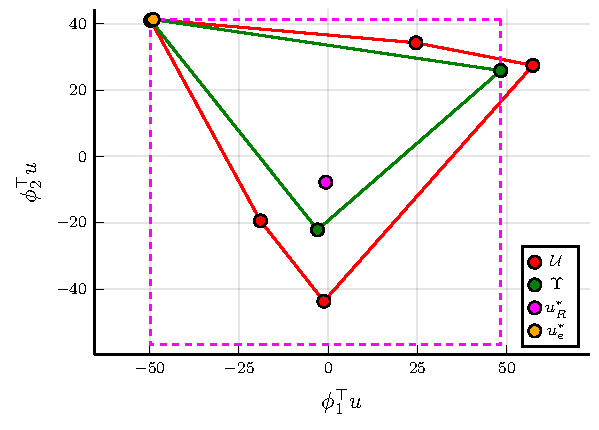
\includegraphics[width=0.95\textwidth, height=0.85\textheight]{../../pres_roil/plots/visual_solve_cheb.pdf}
  \end{center}
\end{frame}

\section*{Experiments}

\begin{frame}
\frametitle{40x40 Gridworld}
\begin{figure}
    \begin{minipage}{0.45\linewidth}
      \centering
      \textbf{On-Policy}
      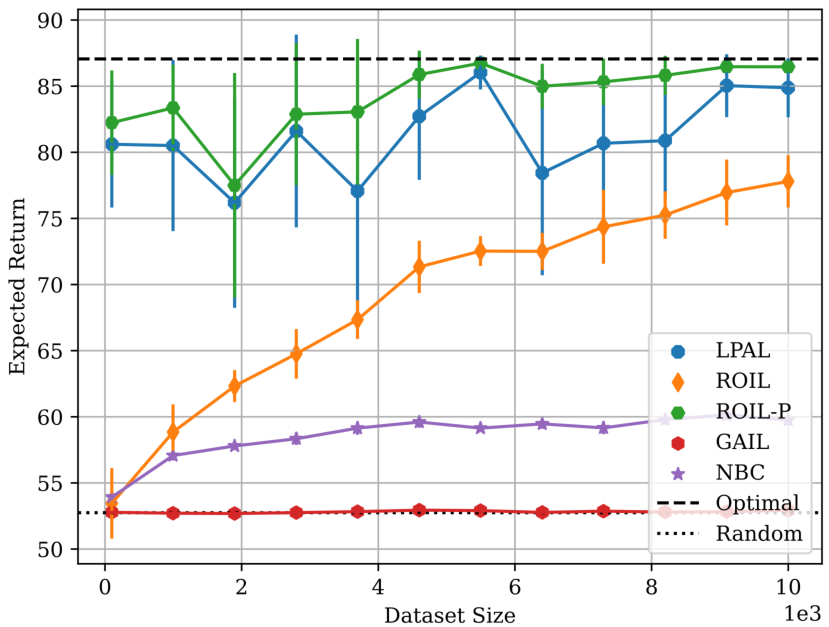
\includegraphics[scale=0.4]{../../pres_roil/plots/returns/40x40_gridworld_on_policy_returns_cropped.pdf}
    \end{minipage}
    \hspace{0.06\linewidth}
    \begin{minipage}{0.45\linewidth}
      \centering
      \textbf{Off-Policy}
      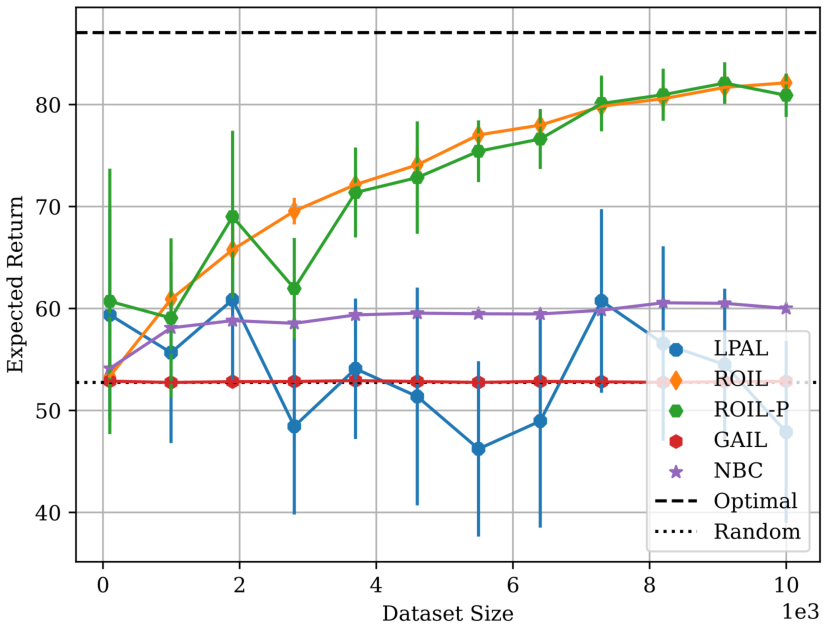
\includegraphics[scale=0.4]{../../pres_roil/plots/returns/40x40_gridworld_off_policy_returns_cropped.pdf}
    \end{minipage}
\end{figure}
\end{frame}

% \begin{frame}
% \frametitle{Regret Comparison}

%  \[ Regret(\pi) = \max_{\pi_e \in \Pi_R(D_e)} \max_{w \in \mathcal{W}} \rho(\pi_e, \Phi w) - \rho(\pi, \Phi w)\]

% \begin{figure}
%   \begin{center}
%   \begin{minipage}{0.47\linewidth}
%     \centering
%     \textbf{On-Policy}
%     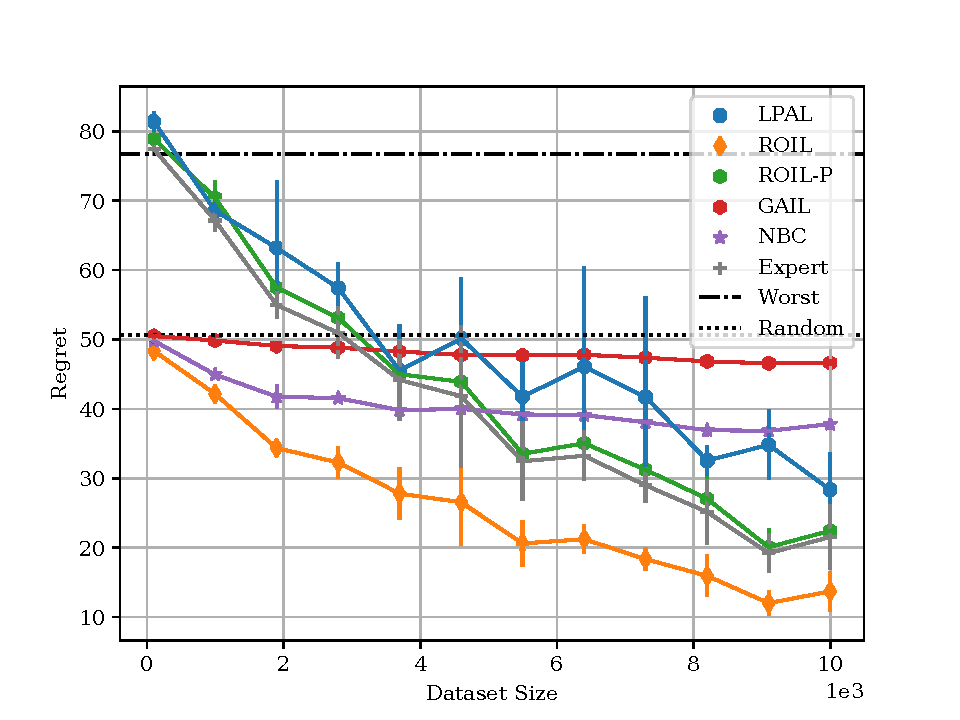
\includegraphics[width=\linewidth]{../../pres_roil/plots/regrets/40x40_gridworld_on_policy_regret_regrets.pdf}
%   \end{minipage}
%   \begin{minipage}{0.47\linewidth}
%     \centering
%     \textbf{Off-Policy}
%     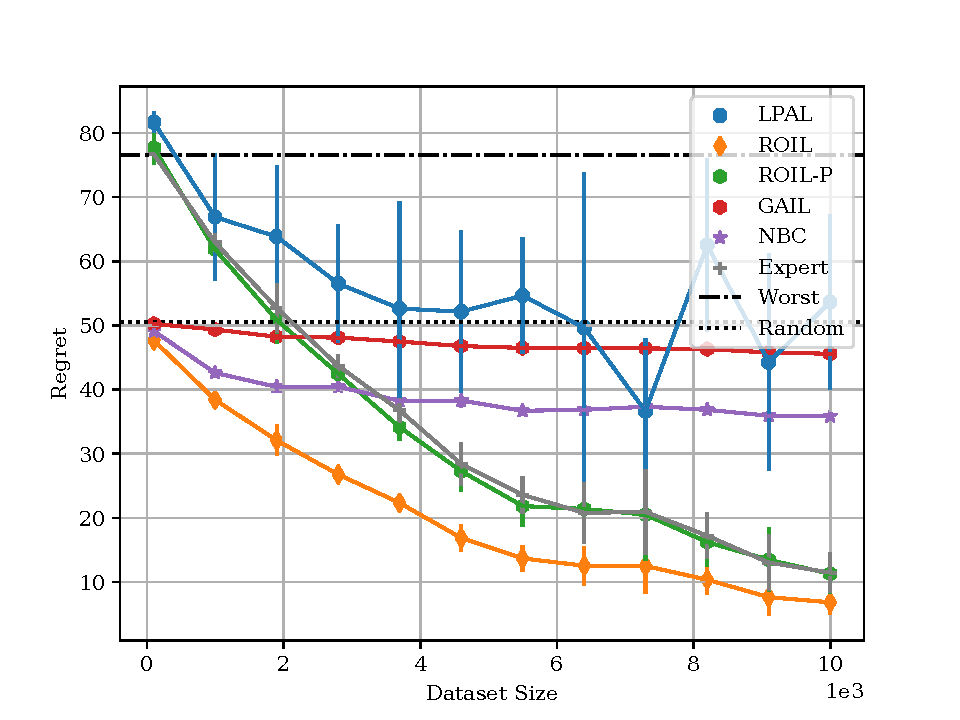
\includegraphics[width=\linewidth]{../../pres_roil/plots/regrets/40x40_gridworld_off_policy_regret_regrets.pdf}
%   \end{minipage}
%   \end{center}
% \end{figure}

% \end{frame}

\section*{Conclusion}

\begin{frame}
	\frametitle{Conclusion}
	\begin{itemize}
    \item Need \emph{off-policy} IRL
    \vfill
    \item Existing methods fail
    \vfill
		\item ROIL outperforms in \emph{off-policy} settings
	\end{itemize}
\end{frame}

\end{document} 
